\section{Used technologies} vue and ts

\subsection{Pinia} - state management
\subsection{Router} - routing 
\subsection{Axios} - be calls

\section{Authentication and authorization}
Authentication and authorization processes are implemented using OAuth 2.0 protocol


\subsection{OAuth protocol and authorization server}
OAuth protocol is a modern industry-standard protocol for authorization. The concept of that protocol is granting access to a user without a need for a user to share their credentials with an application they want to access. It requires an additional authorization server that provides the authentication and authorization processes. We use the faculty authorization server for that purpose.

https://rozvoj.fit.cvut.cz/Main/oauth2


\subsection{Apps manager} In order to start the authorization process using the OAuth protocol we need to resolve the communication with the authorization server. To successfully send the authorization request and then get redirected back to the application after successful authorization, the application needs to be registered in the App Manager.\\
The authorization request, which the frontend sends to the authorization server needs to contain certain parameters: client id, client secret and redirect URL. The first two parameters are generated by the app manager, while the redirect URL can be set to the URL we want to get redirected to after the successful authorization of a user.
%https://auth.fit.cvut.cz/manager/app-types.xhtml

\begin{figure}[hp]
\centering
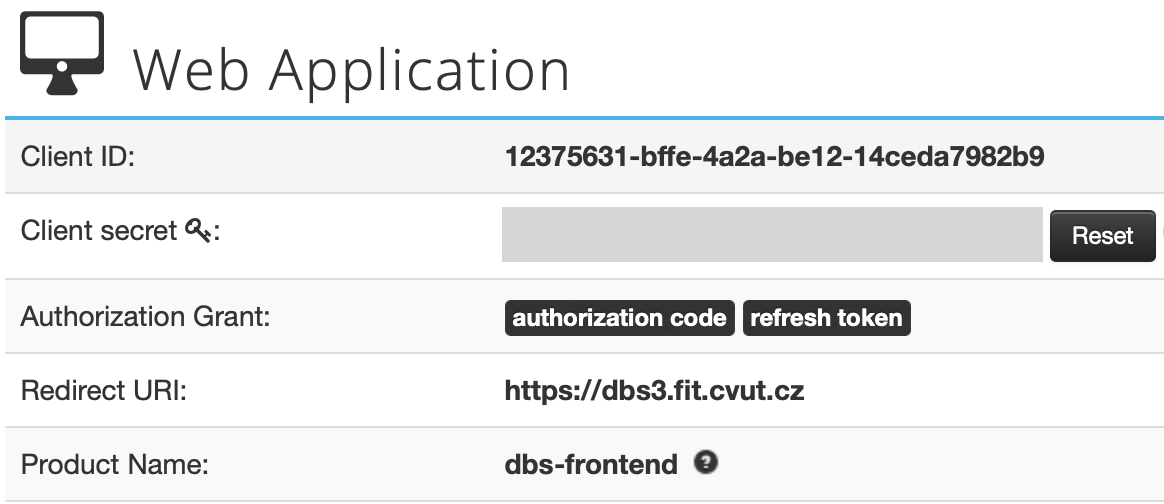
\includegraphics[scale=0.52]{../png/app_manager.png}
\caption{The example of the application registry in the App Manager}
\end{figure}




\subsection{Communication with backend and CORS}


\section{Tokens and security}


all description

\subsection{Access token}
The access token is a short-time living token that is used to verify the user's access to the application on both frontend and backend sides. An access token is sent in every request sent to backend, so backend can verify if the token is valid and only then complete a request.

\paragraph*{JWT token}

\subsection{Refresh token}
The refresh token is meant to be a long-time living token. Because it is supposed to have a longer expiration time to be able to refresh an access token.
However, our microservice supports refresh token rotation, which means that every time we refresh the access token we also get a new refresh token, which makes its time living much shorter and thus more secure. There are different opinions about what is the best and most secure way of storing this token. [OAuth] pages say that with use of token rotation using local storage is possible


\subsection{Security}
Cookies hello , adjustment to microservice 



\section{Role-based access control}

\subsection{Access control for routing}

\subsection{Authentication control for requests}


